\chapter{Efficient computation}\label{chapefficient}

\begin{objectives} \label[objectives]{Describe-at-a-high-level-}

\begin{itemize}
\tightlist
\item
  Describe at a high level some interesting computational problems.\\
\item
  The difference between polynomial and exponential time.\\
\item
  Examples of techniques for obtaining efficient algorithms\\
\item
  Examples of how seemingly small differences in problems can
  potentially make huge differences in their computational complexity.
\end{itemize}

\end{objectives}

\begin{quote}
\emph{``The problem of distinguishing prime numbers from composite and
of resolving the latter into their prime factors is \ldots{} one of the
most important and useful in arithmetic \ldots{} Nevertheless we must
confess that all methods \ldots{} are either restricted to very special
cases or are so laborious \ldots{} they try the patience of even the
practiced calculator \ldots{} and do not apply at all to larger
numbers.''}, Carl Friedrich Gauss, 1798
\end{quote}

\begin{quote}
\emph{``For practical purposes, the difference between algebraic and
exponential order is often more crucial than the difference between
finite and non-finite.''}, Jack Edmunds, ``Paths, Trees, and Flowers'',
1963
\end{quote}

\begin{quote} \label[quote]{What-is-the-most-efficien}

\emph{``What is the most efficient way to sort a million 32-bit
integers?''}, Eric Schmidt to Barack Obama, 2008

\emph{``I think the bubble sort would be the wrong way to go.''}, Barack
Obama.

\end{quote}

So far we have been concerned with which functions are \emph{computable}
and which ones are not. In this chapter we look at the finer question of
the \emph{time} that it takes to compute functions, as a \emph{function
of their input length}. Time complexity is extremely important to both
the theory and practice of computing, but in introductory courses,
coding interviews, and software development, terms such as ``\(O(n)\)
running time'' are often used in an informal way. People don't have a
precise definition of what a linear-time algorithm is, but rather assume
that ``they'll know it when they see it''. In this book we will define
running time precisely, using the mathematical models of computation we
developed in the previous chapters. This will allow us to ask (and
sometimes answer) questions such as:

\begin{itemize}
\item
  ``Is there a function that can be computed in \(O(n^2)\) time but not
  in \(O(n)\) time?''
\item
  ``Are there natural problems for which the \emph{best} algorithm (and
  not just the \emph{best known}) requires \(2^{\Omega(n)}\) time?''
\end{itemize}

\hypertarget{runtimefunc}{}
\begin{bigidea} \label[bigidea]{runtimefunc}

The running time of an algorithm is not a \emph{number}, it is a
\emph{function} of the length of the input.

\end{bigidea}

We will see the precise definition of running time (using Turing
machines and RAM machines / NAND-RAM) in \cref{chapmodelruntime}. In
this chapter, we informally survey examples of computational problems.
For some of these problems we know efficient (i.e., \(O(n^c)\)-time for
a small constant \(c\)) algorithms, and for others the best known
algorithms are \emph{exponential}. We present these examples to get a
feel as to the kinds of problems that lie on each side of this divide
and also see how sometimes seemingly minor changes in problem
formulation can make the (known) complexity of a problem ``jump'' from
polynomial to exponential. We do not formally define the notion of
running time in this chapter, but use the same ``I know it when I see
it'' notion of an \(O(n)\) or \(O(n^2)\) time algorithms as the one
you've seen in introduction to computer science courses.

While the difference between \(O(n)\) and \(O(n^2)\) time can be crucial
in practice, we focus on the difference between \emph{polynomial} and
\emph{exponential} running time. One advantage is that, as we will see,
questions about polynomial versus exponential time are often
\emph{insensitive} to the choice of the particular computational model,
just as the question of whether a function \(F\) is computable is
insensitive to whether you use Turing machines, \(\lambda\)-calculus, or
Javascript as your model of computation. One of the interesting
phenomena of computing is that there is often a kind of a ``threshold
phenomenon'' or ``zero-one law'' for running time. Many natural problems
can either be solved in \emph{polynomial} running time with a
\emph{not-too-large exponent} (e.g., something like \(O(n^2)\) or
\(O(n^3)\)), or require \emph{exponential} (e.g., at least
\(2^{\Omega(n)}\) or \(2^{\Omega(\sqrt{n})}\)) time to solve. The
reasons for this phenomenon are still not fully understood, but some
light on this is shed by the concept of \emph{NP completeness}, which we
will see in \cref{cooklevinchap}.

This chapter is merely a tiny sample of the landscape of computational
problems and efficient algorithms. If you want to explore the field of
algorithms and data structures more deeply (which I very much hope you
do!), the bibliographical notes contain references to some excellent
texts, some of which are available freely on the web.

\hypertarget{relationpartsrem}{}
\begin{remark}[Relations between parts of this book] \label[remark]{relationpartsrem}

\textbf{Part I} of this book contained a \emph{quantitative study} of
computation of \emph{finite functions}. We asked what are the resources
(in terms of gates of Boolean circuits or lines in straight-line
programs) required to compute various finite functions.

\textbf{Part II} of the book contained a \emph{qualitative study} of
computation of \emph{infinite functions} (i.e., functions of
\emph{unbounded input length}). In that part we asked the
\emph{qualitative question} of whether or not a function is computable
at all, regardless of the number of operations.

\textbf{Part III} of the book, beginning with this chapter, merges the
two approaches and contains a \emph{quantitative study} of computation
of \emph{infinite functions}. In this part we ask how do resources for
computing a function \emph{scale} with the length of the input. In
\cref{chapmodelruntime} we define the notion of running time, and the
class \(\mathbf{P}\) of functions that can be computed using a number of
steps that scales \emph{polynomially} with the input length. In
\cref{nonuniformcompsec} we will relate this class to the models of
Boolean circuits and straightline programs that we studied in Part I.

\end{remark}

\section{Problems on graphs}\label{Problems-on-graphs}

In this chapter we discuss several examples of important computational
problems. Many of the problems will involve \emph{graphs}. We have
already encountered graphs before (see \cref{graphsec}) but now quickly
recall the basic notation. A graph \(G\) consists of a set of
\emph{vertices} \(V\) and \emph{edges} \(E\) where each edge is a pair
of vertices. We typically denote by \(n\) the number of vertices (and in
fact often consider graphs where the set of vertices \(V\) equals the
set \([n]\) of the integers between \(0\) and \(n-1\)). In a
\emph{directed} graph, an edge is an ordered pair \((u,v)\), which we
sometimes denote as \(\overrightarrow{u\;v}\). In an \emph{undirected}
graph, an edge is an unordered pair (or simply a set) \(\{ u,v \}\)
which we sometimes denote as \(\overline{u\; v}\) or \(u \sim v\). An
equivalent viewpoint is that an undirected graph corresponds to a
directed graph satisfying the property that whenever the edge
\(\overrightarrow{u\; v}\) is present then so is the edge
\(\overrightarrow{v\; u}\). In this chapter we restrict our attention to
graphs that are undirected and simple (i.e., containing no parallel
edges or self-loops). Graphs can be represented either in the
\emph{adjacency list} or \emph{adjacency matrix} representation. We can
transform between these two representations using \(O(n^2)\) operations,
and hence for our purposes we will mostly consider them as equivalent.

Graphs are so ubiquitous in computer science and other sciences because
they can be used to model a great many of the data that we encounter.
These are not just the ``obvious'' data such as the road network (which
can be thought of as a graph of whose vertices are locations with edges
corresponding to road segments), or the web (which can be thought of as
a graph whose vertices are web pages with edges corresponding to links),
or social networks (which can be thought of as a graph whose vertices
are people and the edges correspond to friend relation). Graphs can also
denote correlations in data (e.g., graph of observations of features
with edges corresponding to features that tend to appear together),
causal relations (e.g., gene regulatory networks, where a gene is
connected to gene products it derives), or the state space of a system
(e.g., graph of configurations of a physical system, with edges
corresponding to states that can be reached from one another in one
step).


\begin{marginfigure}
\centering
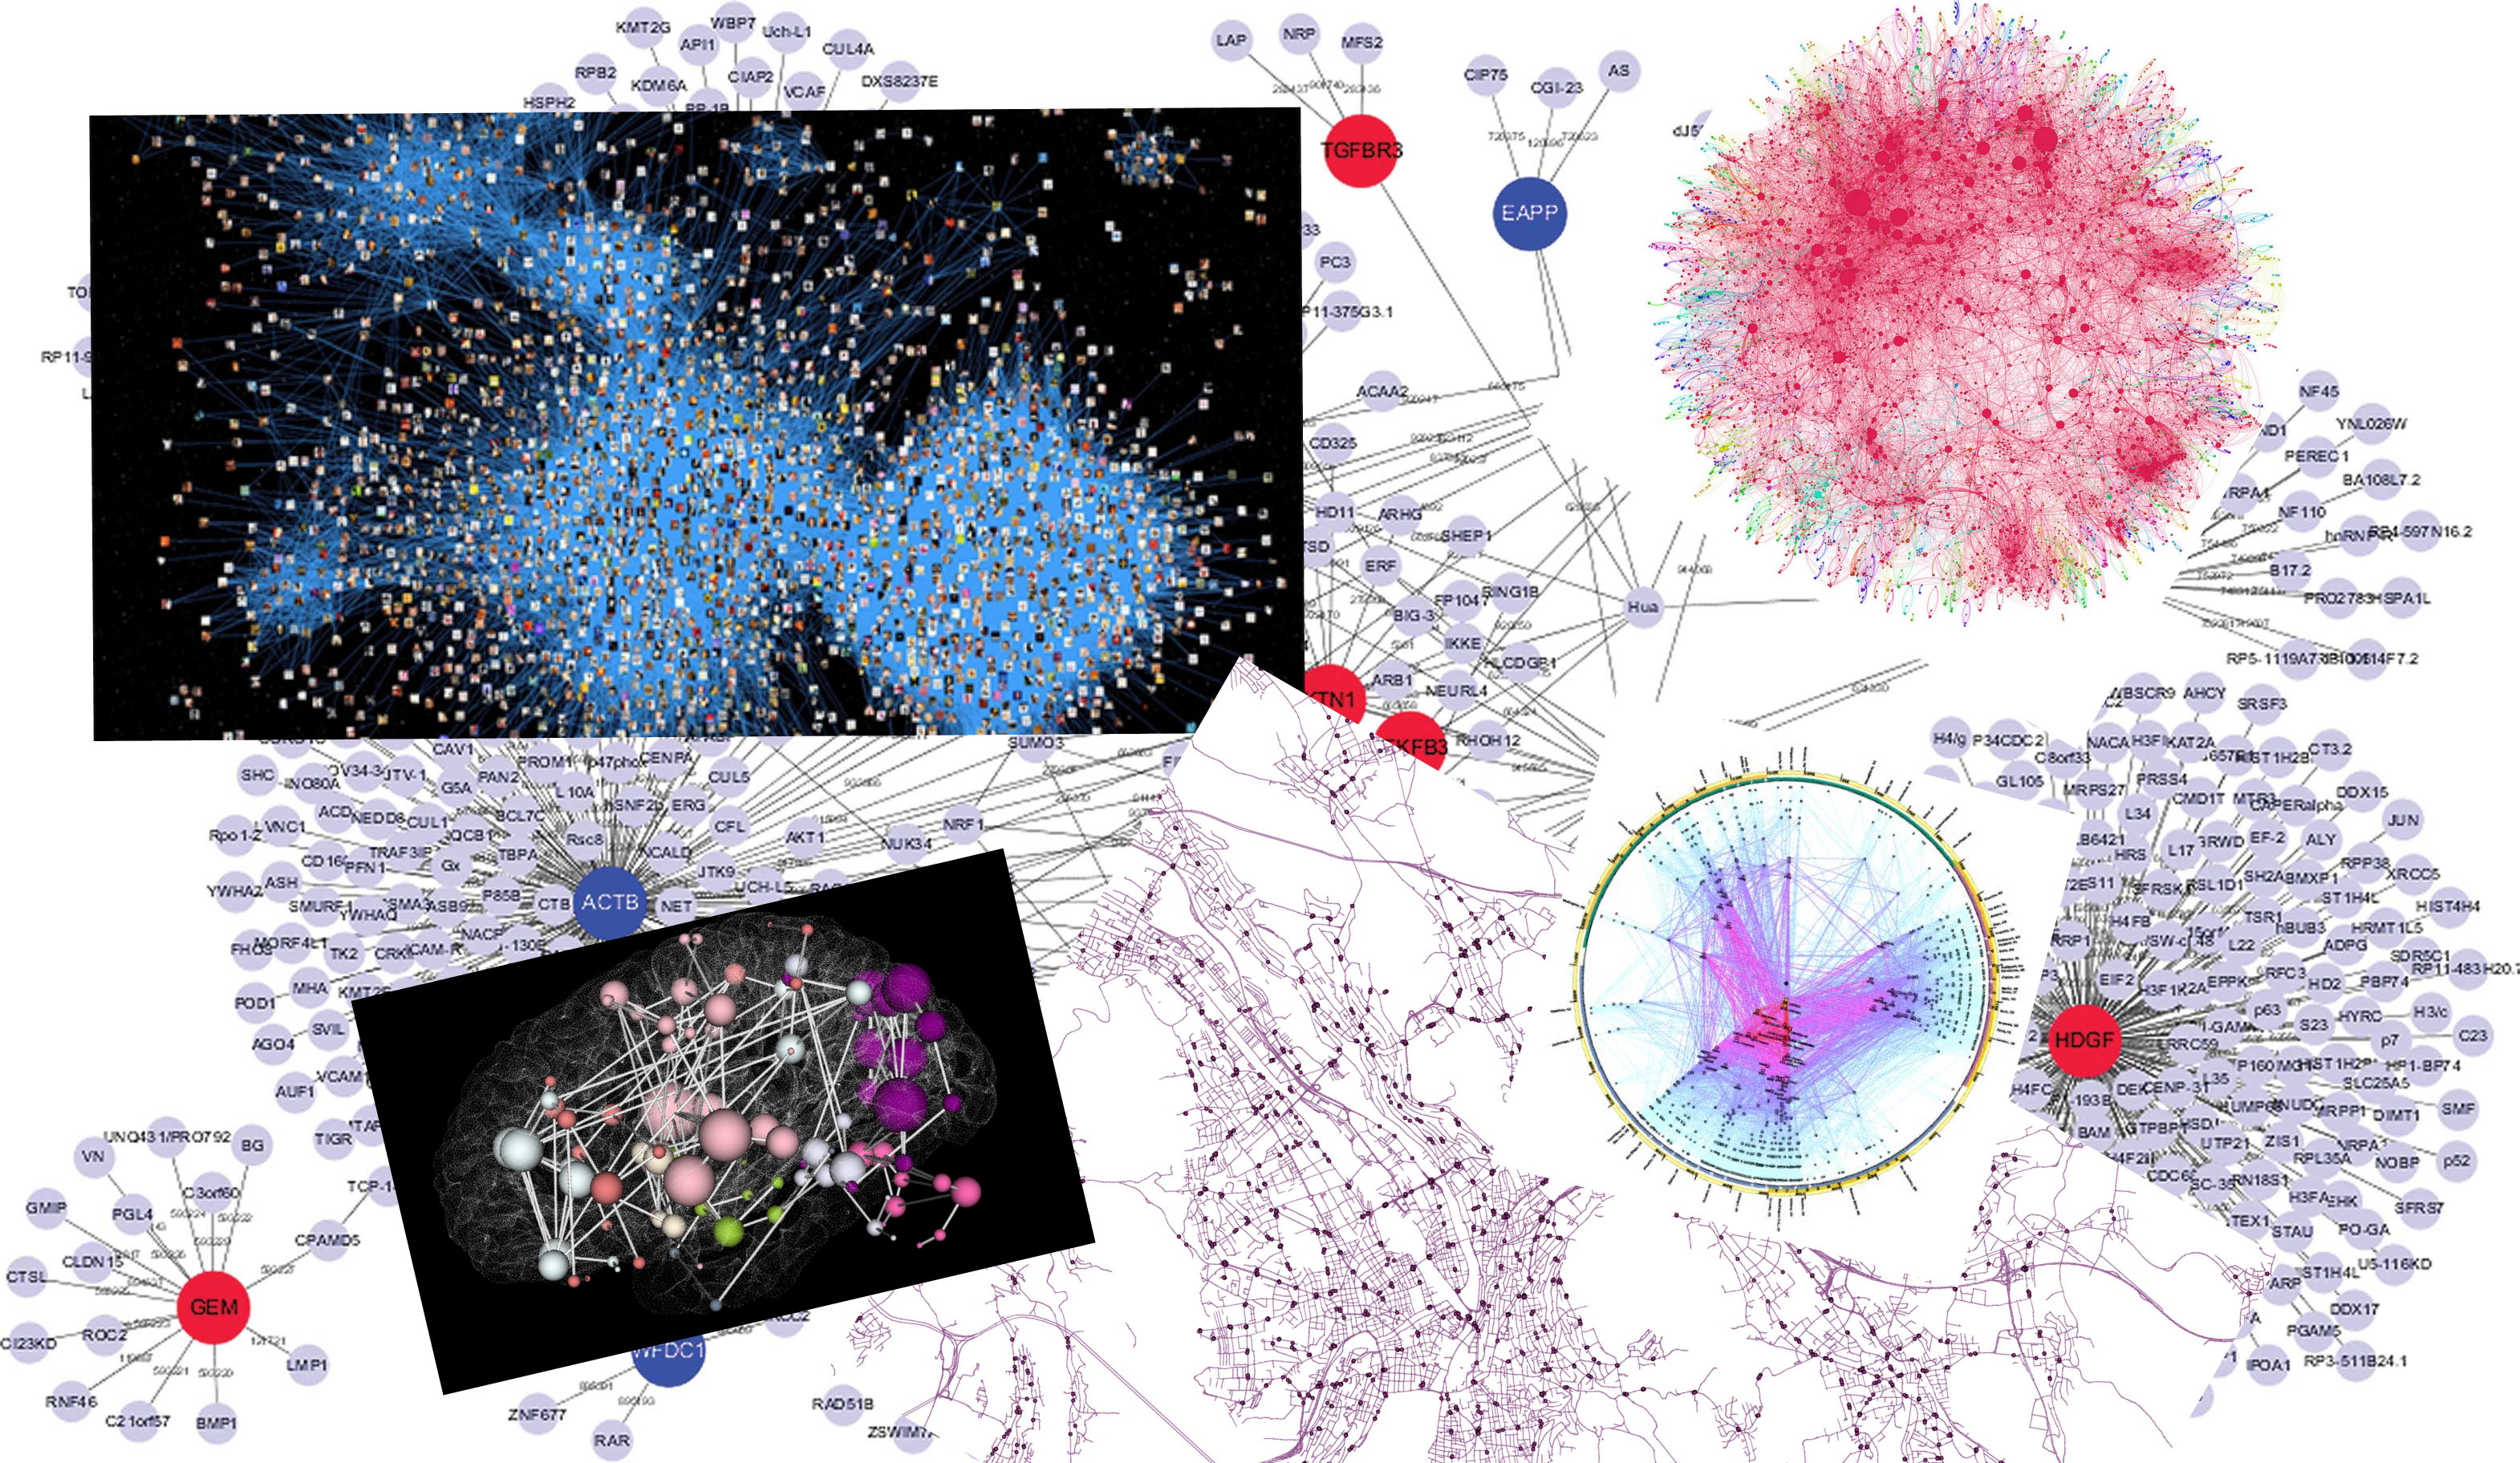
\includegraphics[width=\linewidth, height=1.5in, keepaspectratio]{../figure/graphs.png}
\caption{Some examples of graphs found on the Internet.}
\label{graphsfromwebfig}
\end{marginfigure}

\subsection{Finding the shortest path in a
graph}\label{Finding-the-shortest-path}

The \emph{shortest path problem} is the task of, given a graph
\(G=(V,E)\) and two vertices \(s,t \in V\), to find the length of the
shortest path between \(s\) and \(t\) (if such a path exists). That is,
we want to find the smallest number \(k\) such that there are vertices
\(v_0,v_1,\ldots,v_k\) with \(v_0=s\), \(v_k=t\) and for every
\(i\in\{0,\ldots,k-1\}\) an edge between \(v_i\) and \(v_{i+1}\).
Formally, we define
\(\ensuremath{\mathit{MINPATH}}:\{0,1\}^* \rightarrow \{0,1\}^*\) to be
the function that on input a triple \((G,s,t)\) (represented as a
string) outputs the number \(k\) which is the length of the shortest
path in \(G\) between \(s\) and \(t\) or a string representing
\texttt{no path} if no such path exists. (In practice people often want
to also find the actual path and not just its length; it turns out that
the algorithms to compute the length of the path often yield the actual
path itself as a byproduct, and so everything we say about the task of
computing the length also applies to the task of finding the path.)

If each vertex has at least two neighbors then there can be an
\emph{exponential} number of paths from \(s\) to \(t\), but fortunately
we do not have to enumerate them all to find the shortest path. We can
find the shortest path using a
\href{https://en.wikipedia.org/wiki/Breadth-first_search}{breadth first
search (BFS)}, enumerating \(s\)'s neighbors, and then neighbors'
neighbors, etc.. in order. If we maintain the neighbors in a list we can
perform a BFS in \(O(n^2)\) time, while using a \emph{queue} we can do
this in \(O(m)\) time.\footnote{A \emph{queue} is a data structure for
  storing a list of elements in ``First In First Out (FIFO)'' order.
  Each ``pop'' operation removes an element from the queue in the order
  that they were ``pushed'' into it; see the
  \href{https://goo.gl/HY9BJD}{Wikipedia page}.}
\href{https://goo.gl/PJyc4D}{Dijkstra's algorithm} is a well-known
generalization of BFS to \emph{weighted} graphs. More formally, the
algorithm for computing the function \(\ensuremath{\mathit{MINPATH}}\)
is described in \cref{bfsshortpathalg}.

\begin{algorithm}[Shortest path via BFS]
\label[algorithm]{bfsshortpathalg} ~ \\ \noindent
\begin{algorithmic}[1]
\INPUT  Graph $G=(V,E)$ and vertices $s,t\in V$. Assume $V=[n]$.
\OUTPUT  Length $k$ of shortest path from $s$ to $t$ or  $\infty$ if no such path exists.
\STATE Let $D$ be length-$n$ array. 
\STATE Set $D[s]=0$ and $D[i]=\infty$ for all $i\in [n] \setminus \{s \}$.
\STATE Initialize queue $Q$ to contain $s$.
\WHILE{$S$ non empty}
\STATE Pop $v$ from $Q$
\IF{$v=t$}
\RETURN $D[v]$
\ENDIF
\FOR{$u$ neighbor of $v$ with $D[u]=\infty$}
   \STATE Set $D[u] \leftarrow D[v]+1$
   \STATE Add $u$ to $Q$.
\ENDFOR
\ENDWHILE
\RETURN $\infty$
\end{algorithmic}
\end{algorithm}

Since we only add to the queue vertices \(w\) with \(D[w]=\infty\) (and
then immediately set \(D[w]\) to an actual number), we never push to the
queue a vertex more than once, and hence the algorithm makes at most
\(n\) ``push'' and ``pop'' operations. For each vertex \(v\), the number
of times we run the inner loop is equal to the \emph{degree} of \(v\)
and hence the total running time is proportional to the sum of all
degrees which equals twice the number \(m\) of edges.
\cref{bfsshortpathalg} returns the correct answer since the vertices are
added to the queue in the order of their distance from \(s\), and hence
we will reach \(t\) after we have explored all the vertices that are
closer to \(s\) than \(t\).

\hypertarget{datastructuresrem}{}
\begin{remark}[On data structures] \label[remark]{datastructuresrem}

If you've ever taken an algorithms course, you have probably encountered
many \emph{data structures} such as \textbf{lists}, \textbf{arrays},
\textbf{queues}, \textbf{stacks}, \textbf{heaps}, \textbf{search trees},
\textbf{hash tables} and many more. Data structures are extremely
important in computer science, and each one of those offers different
tradeoffs between overhead in storage, operations supported, cost in
time for each operation, and more. For example, if we store \(n\) items
in a list, we will need a linear (i.e., \(O(n)\) time) scan to retrieve
an element, while we achieve the same operation in \(O(1)\) time if we
used a hash table. However, when we only care about polynomial-time
algorithms, such factors of \(O(n)\) in the running time will not make
much difference. Similarly, if we don't care about the difference
between \(O(n)\) and \(O(n^2)\), then it doesn't matter if we represent
graphs as adjacency lists or adjacency matrices. Hence we will often
describe our algorithms at a very high level, without specifying the
particular data structures that are used to implement them. However, it
will always be clear that there exists \emph{some} data structure that
is sufficient for our purposes.

\end{remark}

\subsection{Finding the longest path in a
graph}\label{Finding-the-longest-path-}

The \emph{longest path problem} is the task of finding the length of the
\emph{longest} simple (i.e., non intersecting) path between a given pair
of vertices \(s\) and \(t\) in a given graph \(G\). If the graph is a
road network, then the longest path might seem less motivated than the
shortest path (unless you are the kind of person that always prefers the
``scenic route''). But of graphs can and are used to model a variety of
phenomena, and in many such cases finding the longest path (and some of
its variants) can be very useful. In particular, finding the longest
path is a generalization of the famous
\href{https://en.wikipedia.org/wiki/Hamiltonian_path_problem}{Hamiltonian
path problem} which asks for a \emph{maximally long} simple path (i.e.,
path that visits all \(n\) vertices once) between \(s\) and \(t\), as
well as the notorious
\href{https://en.wikipedia.org/wiki/Travelling_salesman_problem}{traveling
salesman problem (TSP)} of finding (in a weighted graph) a path visiting
all vertices of cost at most \(w\). TSP is a classical optimization
problem, with applications ranging from planning and logistics to DNA
sequencing and astronomy.

Surprisingly, while we can find the shortest path in \(O(m)\) time,
there is no known algorithm for the \emph{longest path problem} that
significantly improves on the trivial ``exhaustive search'' or ``brute
force'' algorithm that enumerates all the exponentially many
possibilities for such paths. Specifically, the best known algorithms
for the longest path problem take \(O(c^n)\) time for some constant
\(c>1\). (At the moment the best record is \(c \sim 1.65\) or so; even
obtaining an \(O(2^n)\) time bound is not that simple, see
\cref{longest-path-ex}.)


\begin{marginfigure}
\centering
\includegraphics[width=\linewidth, height=1.5in, keepaspectratio]{../figure/knights_tour.jpg}
\caption{A \emph{knight's tour} can be thought of as a maximally long
path on the graph corresponding to a chessboard where we put an edge
between any two squares that can be reached by one step via a legal
knight move.}
\label{knighttourpath}
\end{marginfigure}

\subsection{Finding the minimum cut in a graph}\label{mincutsec}

Given a graph \(G=(V,E)\), a \emph{cut} of \(G\) is a subset
\(S \subseteq V\) such that \(S\) is neither empty nor is it all of
\(V\). The edges cut by \(S\) are those edges where one of their
endpoints is in \(S\) and the other is in
\(\overline{S} = V \setminus S\). We denote this set of edges by
\(E(S,\overline{S})\). If \(s,t \in V\) are a pair of vertices then an
\emph{\(s,t\) cut} is a cut such that \(s\in S\) and
\(t\in \overline{S}\) (see \cref{cutingraphfig}). The \emph{minimum
\(s,t\) cut problem} is the task of finding, given \(s\) and \(t\), the
minimum number \(k\) such that there is an \(s,t\) cut cutting \(k\)
edges (the problem is also sometimes phrased as finding the set that
achieves this minimum; it turns out that algorithms to compute the
number often yield the set as well). Formally, we define
\(\ensuremath{\mathit{MINCUT}}:\{0,1\}^* \rightarrow \{0,1\}^*\) to be
the function that on input a string representing a triple
\((G=(V,E),s,t)\) of a graph and two vertices, outputs the minimum
number \(k\) such that there exists a set \(S \subseteq V\) with
\(s\in S\), \(t\not\in S\) and \(|E(S,\overline{S})|=k\).


\begin{marginfigure}
\centering
\includegraphics[width=\linewidth, height=1.5in, keepaspectratio]{../figure/cutingraph.png}
\caption{A \emph{cut} in a graph \(G=(V,E)\) is simply a subset \(S\) of
its vertices. The edges that are \emph{cut} by \(S\) are all those whose
one endpoint is in \(S\) and the other one is in
\(\overline{S} = V \setminus S\). The cut edges are colored red in this
figure.}
\label{cutingraphfig}
\end{marginfigure}

Computing minimum \(s,t\) cuts is useful for in many applications since
minimum cuts often correspond to \emph{bottlenecks}. For example, in a
communication or railroad network the minimum cut between \(s\) and
\(t\) corresponds to the smallest number of edges that, if dropped, will
disconnect \(s\) from \(t\). (This was actually the original motivation
for this problem; see \cref{effalgnotes}.) Similar applications arise in
scheduling and planning. In the setting of
\href{https://en.wikipedia.org/wiki/Image_segmentation}{image
segmentation}, one can define a graph whose vertices are pixels and
whose edges correspond to neighboring pixels of distinct colors. If we
want to separate the foreground from the background then we can pick (or
guess) a foreground pixel \(s\) and background pixel \(t\) and ask for a
minimum cut between them.

The naive algorithm for computing \(\ensuremath{\mathit{MINCUT}}\) will
check all \(2^n\) possible subsets of an \(n\)-vertex graph, but it
turns out we can do much better than that. As we've seen in this book
time and again, there is more than one algorithm to compute the same
function,and some of those algorithms might be more efficient than
others. Luckily the minimum cut problem is one of those cases. In
particular, as we will see in the next section, there are algorithms
that compute \(\ensuremath{\mathit{MINCUT}}\) in time which is
\emph{polynomial} in the number of vertices.

\subsection{Min-Cut Max-Flow and Linear programming}\label{linerprogsec}

We can obtain a polynomial-time algorithm for computing
\(\ensuremath{\mathit{MINCUT}}\) using the
\href{https://en.wikipedia.org/wiki/Max-flow_min-cut_theorem}{Max-Flow
Min-Cut Theorem}. This theorem says that the minimum cut between \(s\)
and \(t\) equals the maximum amount of \emph{flow} we can send from
\(s\) to \(t\), if every edge has unit capacity. Specifically, imagine
that every edge of the graph corresponded to a pipe that could carry one
unit of fluid per one unit of time (say 1 liter of water per second).
The \emph{maximum \(s,t\) flow} is the maximum units of water that we
could transfer from \(s\) to \(t\) over these pipes. If there is an
\(s,t\) cut of \(k\) edges, then the maximum flow is at most \(k\). The
reason is that such a cut \(S\) acts as a ``bottleneck'' since at most
\(k\) units can flow from \(S\) to its complement at any given unit of
time. This means that the maximum \(s,t\) flow is always \emph{at most}
the value of the minimum \(s,t\) cut. The surprising and non-trivial
content of the Max-Flow Min-Cut Theorem is that the maximum flow is also
\emph{at least} the value of the minimum cut, and hence computing the
cut is the same as computing the flow.

The Max-Flow Min-Cut Theorem reduces the task of computing a minimum cut
to the task of computing a \emph{maximum flow}. However, this still does
not show how to compute such a flow. The
\href{https://en.wikipedia.org/wiki/Ford\%E2\%80\%93Fulkerson_algorithm}{Ford-Fulkerson
Algorithm} is a direct way to compute a flow using incremental
improvements. But computing flows in polynomial time is also a special
case of a much more general tool known as
\href{https://en.wikipedia.org/wiki/Linear_programming}{linear
programming}.

A \emph{flow} on a graph \(G\) of \(m\) edges can be modeled as a vector
\(x\in \R^m\) where for every edge \(e\), \(x_e\) corresponds to the
amount of water per time-unit that flows on \(e\). We think of an edge
\(e\) an an ordered pair \((u,v)\) (we can choose the order arbitrarily)
and let \(x_e\) be the amount of flow that goes from \(u\) to \(v\). (If
the flow is in the other direction then we make \(x_e\) negative.) Since
every edge has capacity one, we know that \(-1 \leq x_e \leq 1\) for
every edge \(e\). A valid flow has the property that the amount of water
leaving the source \(s\) is the same as the amount entering the sink
\(t\), and that for every other vertex \(v\), the amount of water
entering and leaving \(v\) is the same.

Mathematically, we can write these conditions as follows:

\[
\begin{aligned}
\sum_{e \ni s} x_e  + \sum_{e\ni t} x_e &=0  && \\
\sum_{e\ni v} x_e &=0 \; &&\forall_{v \in V \setminus \{s,t\}} \\
-1 \leq x_e \leq 1 &  \; &&\forall_{e\in E}
\end{aligned}
\label{eqlinprogmincut}
\] where for every vertex \(v\), summing over \(e \ni v\) means summing
over all the edges that touch \(v\).

The maximum flow problem can be thought of as the task of maximizing
\(\sum_{e \ni s} x_e\) over all the vectors \(x\in\R^m\) that satisfy
the above conditions \eqref{eqlinprogmincut}. Maximizing a linear
function \(\ell(x)\) over the set of \(x\in \R^m\) that satisfy certain
linear equalities and inequalities is known as \emph{linear
programming}. Luckily, there are
\href{https://en.wikipedia.org/wiki/Linear_programming\#Algorithms}{polynomial-time
algorithms} for solving linear programming, and hence we can solve the
maximum flow (and so, equivalently, minimum cut) problem in polynomial
time. In fact, there are much better algorithms for
maximum-flow/minimum-cut, even for weighted directed graphs, with
currently the record standing at \(O(\min\{ m^{10/7}, m\sqrt{n}\})\)
time.

\hypertarget{globalmincut}{}
\begin{solvedexercise}[Global minimum cut] \label[solvedexercise]{globalmincut}

Given a graph \(G=(V,E)\), define the \emph{global} minimum cut of \(G\)
to be the minimum over all \(S \subseteq V\) with \(S \neq \emptyset\)
and \(S \neq V\) of the number of edges cut by \(S\). Prove that there
is a polynomial-time algorithm to compute the global minimum cut of a
graph.

\end{solvedexercise}

\begin{solution} \label[solution]{By-the-above-we-know-that}

By the above we know that there is a polynomial-time algorithm \(A\)
that on input \((G,s,t)\) finds the minimum \(s,t\) cut in the graph
\(G\). Using \(A\), we can obtain an algorithm \(B\) that on input a
graph \(G\) computes the global minimum cut as follows:

\begin{enumerate}
\def\labelenumi{\arabic{enumi}.}
\item
  For every distinct pair \(s,t \in V\), Algorithms \(B\) sets
  \(k_{s,t}\leftarrow A(G,s,t)\).
\item
  \(B\) returns the minimum of \(k_{s,t}\) over all distinct pairs
  \(s,t\)
\end{enumerate}

The running time of \(B\) will be \(O(n^2)\) times the running time of
\(A\) and hence polynomial time. Moreover, if the the global minimum cut
is \(S\), then when \(B\) reaches an iteration with \(s\in S\) and
\(t\not\in S\) it will obtain the value of this cut, and hence the value
output by \(B\) will be the value of the global minimum cut.

The above is our first example of a \emph{reduction} in the context of
polynomial-time algorithms. Namely, we reduced the task of computing the
global minimum cut to the task of computing minimum \(s,t\) cuts.

\end{solution}

\subsection{Finding the maximum cut in a
graph}\label{Finding-the-maximum-cut-i}

The \emph{maximum cut} problem is the task of finding, given an input
graph \(G=(V,E)\), the subset \(S\subseteq V\) that \emph{maximizes} the
number of edges cut by \(S\). (We can also define an \(s,t\)-cut variant
of the maximum cut like we did for minimum cut; the two variants have
similar complexity but the global maximum cut is more common in the
literature.) Like its cousin the minimum cut problem, the maximum cut
problem is also very well motivated. For example, maximum cut arises in
VLSI design, and also has some surprising relation to analyzing the
\href{https://en.wikipedia.org/wiki/Ising_model}{Ising model} in
statistical physics.

Surprisingly, while (as we've seen) there is a polynomial-time algorithm
for the minimum cut problem, there is no known algorithm solving
\emph{maximum cut} much faster than the trivial ``brute force''
algorithm that tries all \(2^n\) possibilities for the set \(S\).

\subsection{A note on convexity}\label{A-note-on-convexity}


\begin{marginfigure}
\centering
\includegraphics[width=\linewidth, height=1.5in, keepaspectratio]{../figure/convexvsnot.png}
\caption{In a \emph{convex} function \(f\) (left figure), for every
\(x\) and \(y\) and \(p\in [0,1]\) it holds that
\(f(px+(1-p)y) \leq p\cdot f(x)+(1-p)\cdot f(y)\). In particular this
means that every \emph{local minimum} of \(f\) is also a \emph{global
minimum}. In contrast in a \emph{non convex} function there can be many
local minima.}
\label{convexdeffig}
\end{marginfigure}


\begin{marginfigure}
\centering
\includegraphics[width=\linewidth, height=1.5in, keepaspectratio]{../figure/convexandnon.jpg}
\caption{In the high dimensional case, if \(f\) is a \emph{convex}
function (left figure) the global minimum is the only local minimum, and
we can find it by a local-search algorithm which can be thought of as
dropping a marble and letting it ``slide down'' until it reaches the
global minimum. In contrast, a non-convex function (right figure) might
have an exponential number of local minima in which any local-search
algorithm could get stuck.}
\label{convexfunctionfig}
\end{marginfigure}

There is an underlying reason for the sometimes radical difference
between the difficulty of maximizing and minimizing a function over a
domain. If \(D \subseteq \R^n\), then a function \(f:D \rightarrow R\)
is \emph{convex} if for every \(x,y \in D\) and \(p\in [0,1]\)
\(f(px+(1-p)y) \leq pf(x) + (1-p)f(y)\). That is, \(f\) applied to the
\(p\)-weighted midpoint between \(x\) and \(y\) is smaller than the
\(p\)-weighted average value of \(f\). If \(D\) itself is convex (which
means that if \(x,y\) are in \(D\) then so is the line segment between
them), then this means that if \(x\) is a \emph{local minimum} of \(f\)
then it is also a \emph{global minimum}. The reason is that if
\(f(y)<f(x)\) then every point \(z=px+(1-p)y\) on the line segment
between \(x\) and \(y\) will satisfy
\(f(z) \leq p f(x) + (1-p)f(y) < f(x)\) and hence in particular \(x\)
cannot be a local minimum. Intuitively, local minima of functions are
much easier to find than global ones: after all, any ``local search''
algorithm that keeps finding a nearby point on which the value is lower,
will eventually arrive at a local minima. One example of such a local
search algorithm is
\href{https://en.wikipedia.org/wiki/Gradient_descent}{gradient descent}
which takes a sequence of small steps, each one in the direction that
would reduce the value by the most amount based on the current
derivative.

Indeed, under certain technical conditions, we can often efficiently
find the minimum of convex functions over a convex domain, and this is
the reason why problems such as minimum cut and shortest path are easy
to solve. On the other hand, \emph{maximizing} a convex function over a
convex domain (or equivalently, minimizing a \emph{concave} function)
can often be a hard computational task. A \emph{linear} function is both
convex and concave, which is the reason that both the maximization and
minimization problems for linear functions can be done efficiently.

The minimum cut problem is not a priori a convex minimization task,
because the set of potential cuts is \emph{discrete} and not continuous.
However, it turns out that we can embed it in a continuous and convex
set via the (linear) maximum flow problem. The ``max flow min cut''
theorem ensuring that this embedding is ``tight'' in the sense that the
minimum ``fractional cut'' that we obtain through the maximum-flow
linear program will be the same as the true minimum cut. Unfortunately,
we don't know of such a tight embedding in the setting of the
\emph{maximum} cut problem.

Convexity arises time and again in the context of efficient computation.
For example, one of the basic tasks in machine learning is
\emph{empirical risk minimization}. This is the task of finding a
classifier for a given set of \emph{training examples}. That is, the
input is a list of labeled examples
\((x_{m-1},y_{m-1}),\ldots,(x_{m-1},y_{m-1})\), where each
\(x_i \in \{0,1\}^n\) and \(y_i \in \{0,1\}\), and the goal is to find a
\emph{classifier} \(h:\{0,1\}^n \rightarrow \{0,1\}\) (or sometimes
\(h:\{0,1\}^n \rightarrow \R\)) that minimizes the number of
\emph{errors}. More generally, we want to find \(h\) that minimizes \[
\sum_{i=0}^{m-1}L(y_i,h(x_i))
\] where \(L\) is some \emph{loss function} measuring how far is the
predicted label \(h(x_i)\) from the true label \(y_i\). When \(L\) is
the \emph{square loss} function \(L(y,y')=(y-y')^2\) and \(h\) is a
\emph{linear function}, empirical risk minimization corresponds to the
well-known convex minimization task of \emph{linear regression}. In
other cases, when the task is \emph{non convex}, there can be many
global or local minima. That said, even if we don't find the global (or
even a local) minima, this continuous embedding can still help us. In
particular, when running a local improvement algorithm such as Gradient
Descent, we might still find a function \(h\) that is ``useful'' in the
sense of having a small error on future examples from the same
distribution.

\section{Beyond graphs}\label{Beyond-graphs}

Not all computational problems arise from graphs. We now list some other
examples of computational problems that are of great interest.

\subsection{SAT}\label{SAT}

A \emph{propositional formula} \(\varphi\) involves \(n\) variables
\(x_1,\ldots,x_n\) and the logical operators AND (\(\wedge\)), OR
(\(\vee\)), and NOT (\(\neg\), also denoted as \(\overline{\cdot}\)). We
say that such a formula is in \emph{conjunctive normal form} (CNF for
short) if it is an AND of ORs of variables or their negations (we call a
term of the form \(x_i\) or \(\overline{x}_i\) a \emph{literal}). For
example, this is a CNF formula \[
(x_7 \vee \overline{x}_{22} \vee x_{15} ) \wedge (x_{37} \vee x_{22}) \wedge (x_{55} \vee \overline{x}_7)
\]

The \emph{satisfiability problem} is the task of determining, given a
CNF formula \(\varphi\), whether or not there exists a \emph{satisfying
assignment} for \(\varphi\). A satisfying assignment for \(\varphi\) is
a string \(x\in \{0,1\}^n\) such that if \(\varphi\) evaluates to
\emph{True} if we assign its variables the values of \(x\). The SAT
problem might seem as an abstract question of interest only in logic but
in fact SAT is of huge interest in industrial optimization, with
applications including manufacturing planning, circuit synthesis,
software verification, air-traffic control, scheduling sports
tournaments, and more.

\paragraph{2SAT.} We say that a formula is a \(k\)-CNF it is an AND of
ORs where each OR involves exactly \(k\) literals. The \(k\)-SAT problem
is the restriction of the satisfiability problem for the case that the
input formula is a \(k\)-CNF. In particular, the \emph{2SAT problem} is
to find out, given a \(2\)-CNF formula \(\varphi\), whether there is an
assignment \(x\in \{0,1\}^n\) that \emph{satisfies} \(\varphi\), in the
sense that it makes it evaluate to \(1\) or ``True''. The trivial,
brute-force, algorithm for 2SAT will enumerate all the \(2^n\)
assignments \(x\in \{0,1\}^n\) but fortunately we can do much better.
The key is that we can think of every constraint of the form
\(\ell_i \vee \ell_j\) (where \(\ell_i,\ell_j\) are \emph{literals},
corresponding to variables or their negations) as an \emph{implication}
\(\overline{\ell}_i \Rightarrow \ell_j\), since it corresponds to the
constraints that if the literal \(\ell'_i = \overline{\ell}_i\) is true
then it must be the case that \(\ell_j\) is true as well. Hence we can
think of \(\varphi\) as a directed graph between the \(2n\) literals,
with an edge from \(\ell_i\) to \(\ell_j\) corresponding to an
implication from the former to the latter. It can be shown that
\(\varphi\) is unsatisfiable if and only if there is a variable \(x_i\)
such that there is a directed path from \(x_i\) to \(\overline{x}_i\) as
well as a directed path from \(\overline{x}_i\) to \(x_i\) (see
\cref{twosat_ex}). This reduces 2SAT to the (efficiently solvable)
problem of determining connectivity in directed graphs.

\paragraph{3SAT.} The 3SAT problem is the task of determining
satisfiability for 3CNFs. One might think that changing from two to
three would not make that much of a difference for complexity. One would
be wrong. Despite much effort, we do not know of a significantly better
than brute force algorithm for 3SAT (the best known algorithms take
roughly \(1.3^n\) steps).

Interestingly, a similar issue arises time and again in computation,
where the difference between two and three often corresponds to the
difference between tractable and intractable. We do not fully understand
the reasons for this phenomenon, though the notions of \(\mathbf{NP}\)
completeness we will see later does offer a partial explanation. It may
be related to the fact that optimizing a polynomial often amounts to
equations on its derivative. The derivative of a quadratic polynomial is
linear, while the derivative of a cubic is quadratic, and, as we will
see, the difference between solving linear and quadratic equations can
be quite profound.

\subsection{Solving linear equations}\label{Solving-linear-equations}

One of the most useful problems that people have been solving time and
again is solving \(n\) linear equations in \(n\) variables. That is,
solve equations of the form

\[
\begin{aligned}
a_{0,0}x_0 &+ a_{0,1}x_1 &&+ \cdots &&+ a_{0,{n-1}}x_{n-1} &&= b_0 \\
a_{1,0}x_0 &+ a_{1,1}x_1 &&+ \cdots &&+ a_{1,{n-1}}x_{n-1} &&= b_1 \\
\vdots     &+ \vdots     &&+  \vdots &&+ \vdots              &&= \vdots \\
a_{n-1,0}x_0 &+ a_{n-1,1}x_1 &&+ \cdots &&+ a_{n-1,{n-1}}x_{n-1} &&= b_{n-1}
\end{aligned}
\]

where \(\{ a_{i,j} \}_{i,j \in [n]}\) and \(\{ b_i \}_{i\in [n]}\) are
real (or rational) numbers. More compactly, we can write this as the
equations \(Ax = b\) where \(A\) is an \(n\times n\) matrix, and we
think of \(x,b\) are column vectors in \(\R^n\).

The standard
\href{https://en.wikipedia.org/wiki/Gaussian_elimination}{Gaussian
elimination} algorithm can be used to solve such equations in polynomial
time (i.e., determine if they have a solution, and if so, to find it).
As we discussed above, if we are willing to allow some loss in
precision, we even have algorithms that handle linear
\emph{inequalities}, also known as linear programming. In contrast, if
we insist on \emph{integer} solutions, the task of solving for linear
equalities or inequalities is known as
\href{https://en.wikipedia.org/wiki/Integer_programming}{integer
programming}, and the best known algorithms are exponential time in the
worst case.

\hypertarget{numbersbits}{}
\begin{remark}[Bit complexity of numbers] \label[remark]{numbersbits}

Whenever we discuss problems whose inputs correspond to numbers, the
input length corresponds to how many bits are needed to describe the
number (or, as is equivalent up to a constant factor, the number of
digits in base 10, 16 or any other constant). The difference between the
length of the input and the magnitude of the number itself can be of
course quite profound. For example, most people would agree that there
is a huge difference between having a billion (i.e.~\(10^9\)) dollars
and having nine dollars. Similarly there is a huge difference between an
algorithm that takes \(n\) steps on an \(n\)-bit number and an algorithm
that takes \(2^n\) steps.

One example is the problem (discussed below) of finding the prime
factors of a given integer \(N\). The natural algorithm is to search for
such a factor by trying all numbers from \(1\) to \(N\), but that would
take \(N\) steps which is \emph{exponential} in the input length, which
is the number of bits needed to describe \(N\). (The running time of
this algorithm can be easily improved to roughly \(\sqrt{N}\), but this
is still exponential (i.e., \(2^{n/2}\)) in the number \(n\) of bits to
describe \(N\).) It is an important and long open question whether there
is such an algorithm that runs in time polynomial in the input length
(i.e., polynomial in \(\log N\)).

\end{remark}

\subsection{Solving quadratic
equations}\label{Solving-quadratic-equatio}

Suppose that we want to solve not just \emph{linear} but also equations
involving \emph{quadratic} terms of the form \(a_{i,j,k}x_jx_k\). That
is, suppose that we are given a set of quadratic polynomials
\(p_1,\ldots,p_m\) and consider the equations \(\{ p_i(x) = 0 \}\). To
avoid issues with bit representations, we will always assume that the
equations contain the constraints \(\{ x_i^2 - x_i = 0 \}_{i\in [n]}\).
Since only \(0\) and \(1\) satisfy the equation \(a^2-a\), this
assumption means that we can restrict attention to solutions in
\(\{0,1\}^n\). Solving quadratic equations in several variables is a
classical and extremely well motivated problem. This is the
generalization of the classical case of single-variable quadratic
equations that generations of high school students grapple with. It also
generalizes the
\href{https://www.opt.math.tugraz.at/~cela/papers/qap_bericht.pdf}{quadratic
assignment problem}, introduced in the 1950's as a way to optimize
assignment of economic activities. Once again, we do not know a much
better algorithm for this problem than the one that enumerates over all
the \(2^n\) possibilities.

\section{More advanced examples}\label{More-advanced-examples}

We now list a few more examples of interesting problems that are a
little more advanced but are of significant interest in areas such as
physics, economics, number theory, and cryptography.

\subsection{Determinant of a matrix}\label{Determinant-of-a-matrix}

The \href{https://en.wikipedia.org/wiki/Determinant}{determinant} of a
\(n\times n\) matrix \(A\), denoted by \(\mathrm{det}(A)\), is an
extremely important quantity in linear algebra. For example, it is known
that \(\mathrm{det}(A) \neq 0\) if and only if \(A\) is
\emph{nonsingular}, which means that it has an inverse \(A^{-1}\), and
hence we can always uniquely solve equations of the form \(Ax = b\)
where \(x\) and \(b\) are \(n\)-dimensional vectors. More generally, the
determinant can be thought of as a quantitative measure as to what
extent \(A\) is far from being singular. If the rows of \(A\) are
``almost'' linearly dependent (for example, if the third row is very
close to being a linear combination of the first two rows) then the
determinant will be small, while if they are far from it (for example,
if they are are \emph{orthogonal} to one another, then the determinant
will be large). In particular, for every matrix \(A\), the absolute
value of the determinant of \(A\) is at most the product of the norms
(i.e., square root of sum of squares of entries) of the rows, with
equality if and only if the rows are orthogonal to one another.

The determinant can be defined in several ways. One way to define the
determinant of an \(n\times n\) matrix \(A\) is:

\[
\mathrm{det}(A) = \sum_{\pi \in S_n} \mathrm{sign}(\pi)\prod_{i\in [n]}A_{i,\pi(i)} \label{determinanteq}
\] where \(S_n\) is the set of all permutations from \([n]\) to \([n]\)
and the
\href{https://en.wikipedia.org/wiki/Parity_of_a_permutation}{sign of a
permutation} \(\pi\) is equal to \(-1\) raised to the power of the
number of \emph{inversions} in \(\pi\) (pairs \(i,j\) such that \(i>j\)
but \(\pi(i)<\pi(j)\)).

This definition suggests that computing \(\mathrm{det}(A)\) might
require summing over \(|S_n|\) terms which would take exponential time
since \(|S_n| = n! > 2^n\). However, there are other ways to compute the
determinant. For example, it is known that \(\mathrm{det}\) is the only
function that satisfies the following conditions:

\begin{enumerate}
\def\labelenumi{\arabic{enumi}.}
\item
  \(\mathrm{det}(\ensuremath{\mathit{AB}}) = \mathrm{det}(A)\mathrm{det}(B)\)
  for every square matrices \(A,B\).
\item
  For every \(n\times n\) \emph{triangular} matrix \(T\) with diagonal
  entries \(d_0,\ldots, d_{n-1}\),
  \(\mathrm{det}(T)=\prod_{i=0}^n d_i\). In particular
  \(\mathrm{det}(I)=1\) where \(I\) is the identity matrix. (A
  \emph{triangular} matrix is one in which either all entries below the
  diagonal, or all entries above the diagonal, are zero.)
\item
  \(\mathrm{det}(S)=-1\) where \(S\) is a ``swap matrix'' that
  corresponds to swapping two rows or two columns of \(I\). That is,
  there are two coordinates \(a,b\) such that for every \(i,j\),
  \(S_{i,j} = \begin{cases}1 & i=j\;, i \not\in \{a,b \} \\ 1 & \{i,j\}=\{a,b\} \\ 0 & \text{otherwise}\end{cases}\).
\end{enumerate}

Using these rules and the
\href{https://en.wikipedia.org/wiki/Gaussian_elimination}{Gaussian
elimination} algorithm, it is possible to tell whether \(A\) is singular
or not, and in the latter case, decompose \(A\) as a product of a
polynomial number of swap matrices and triangular matrices. (Indeed one
can verify that the row operations in Gaussian elimination corresponds
to either multiplying by a swap matrix or by a triangular matrix.) Hence
we can compute the determinant for an \(n\times n\) matrix using a
polynomial time of arithmetic operations.

\subsection{Permanent of a matrix}\label{Permanent-of-a-matrix}

Given an \(n\times n\) matrix \(A\), the \emph{permanent} of \(A\) is
defined as

\[
\mathrm{perm}(A) = \sum_{\pi \in S_n} \prod_{i\in [n]}A_{i,\pi(i)} \;. \label{permanenteq} 
\] That is, \(\mathrm{perm}(A)\) is defined analogously to the
determinant in \eqref{determinanteq} except that we drop the term
\(\mathrm{sign}(\pi)\). The permanent of a matrix is a natural quantity,
and has been studied in several contexts including combinatorics and
graph theory. It also arises in physics where it can be used to describe
the quantum state of multiple Boson particles (see
\href{http://www.cs.huji.ac.il/labs/learning/Papers/perm.pdf}{here} and
\href{https://en.wikipedia.org/wiki/Boson_sampling}{here}).

\paragraph{Permanent modulo 2.} If the entries of \(A\) are integers,
then we can define the \emph{Boolean} function \(perm_2\) which outputs
on input a matrix \(A\) the result of the permanent of \(A\) modulo
\(2\). It turns out that we can compute \(perm_2(A)\) in polynomial
time. The key is that modulo \(2\), \(-x\) and \(+x\) are the same
quantity and hence, since the only difference between
\eqref{determinanteq} and \eqref{permanenteq} is that some terms are
multiplied by \(-1\),
\(\mathrm{det}(A) \mod 2 = \mathrm{perm}(A) \mod 2\) for every \(A\).

\paragraph{Permanent modulo 3.} Emboldened by our good fortune above, we
might hope to be able to compute the permanent modulo any prime \(p\)
and perhaps in full generality. Alas, we have no such luck. In a similar
``two to three'' type of a phenomenon, we do not know of a much better
than brute force algorithm to even compute the permanent modulo \(3\).

\subsection{Finding a zero-sum
equilibrium}\label{Finding-a-zero-sum-equili}

A \emph{zero sum game} is a game between two players where the payoff
for one is the same as the penalty for the other. That is, whatever the
first player gains, the second player loses. As much as we want to avoid
them, zero sum games do arise in life, and the one good thing about them
is that at least we can compute the optimal strategy.

A zero sum game can be specified by an \(n\times n\) matrix \(A\), where
if player 1 chooses action \(i\) and player 2 chooses action \(j\) then
player one gets \(A_{i,j}\) and player 2 loses the same amount. The
famous \href{https://en.wikipedia.org/wiki/Min-max_theorem}{Min Max
Theorem} by John von Neumann states that if we allow probabilistic or
``mixed'' strategies (where a player does not choose a single action but
rather a \emph{distribution} over actions) then it does not matter who
plays first and the end result will be the same. Mathematically the min
max theorem is that if we let \(\Delta_n\) be the set of probability
distributions over \([n]\) (i.e., non-negative columns vectors in
\(\R^n\) whose entries sum to \(1\)) then

\[
\max_{p \in \Delta_n} \min_{q\in \Delta_n} p^\top A q =  \min_{q \in \Delta_n} \max_{p\in \Delta_n} p^\top A q \label{eq:minmax}
\]

The min-max theorem turns out to be a corollary of linear programming
duality, and indeed the value of \eqref{eq:minmax} can be computed
efficiently by a linear program.

\subsection{Finding a Nash equilibrium}\label{Finding-a-Nash-equilibriu}

Fortunately, not all real-world games are zero sum, and we do have more
general games, where the payoff of one player does not necessarily equal
the loss of the other.
\href{https://en.wikipedia.org/wiki/John_Forbes_Nash_Jr.}{John Nash} won
the Nobel prize for showing that there is a notion of \emph{equilibrium}
for such games as well. In many economic texts it is taken as an article
of faith that when actual agents are involved in such a game then they
reach a Nash equilibrium. However, unlike zero sum games, we do not know
of an efficient algorithm for finding a Nash equilibrium given the
description of a general (non zero sum) game. In particular this means
that, despite economists' intuitions, there are games for which natural
strategies will take an exponential number of steps to converge to an
equilibrium.

\subsection{Primality testing}\label{Primality-testing}

Another classical computational problem, that has been of interest since
the ancient Greeks, is to determine whether a given number \(N\) is
prime or composite. Clearly we can do so by trying to divide it with all
the numbers in \(2,\ldots,N-1\), but this would take at least \(N\)
steps which is \emph{exponential} in its bit complexity \(n = \log N\).
We can reduce these \(N\) steps to \(\sqrt{N}\) by observing that if
\(N\) is a composite of the form \(N=\ensuremath{\mathit{PQ}}\) then
either \(P\) or \(Q\) is smaller than \(\sqrt{N}\). But this is still
quite terrible. If \(N\) is a \(1024\) bit integer, \(\sqrt{N}\) is
about \(2^{512}\), and so running this algorithm on such an input would
take much more than the lifetime of the universe.

Luckily, it turns out we can do radically better. In the 1970's, Rabin
and Miller gave \emph{probabilistic} algorithms to determine whether a
given number \(N\) is prime or composite in time \(poly(n)\) for
\(n=\log N\). We will discuss the probabilistic model of computation
later in this course. In 2002, Agrawal, Kayal, and Saxena found a
deterministic \(poly(n)\) time algorithm for this problem. This is
surely a development that mathematicians from Archimedes till Gauss
would have found exciting.

\subsection{Integer factoring}\label{Integer-factoring}

Given that we can efficiently determine whether a number \(N\) is prime
or composite, we could expect that in the latter case we could also
efficiently \emph{find} the factorization of \(N\). Alas, no such
algorithm is known. In a surprising and exciting turn of events, the
\emph{non existence} of such an algorithm has been used as a basis for
encryptions, and indeed it underlies much of the security of the world
wide web. We will return to the factoring problem later in this course.
We remark that we do know much better than brute force algorithms for
this problem. While the brute force algorithms would require
\(2^{\Omega(n)}\) time to factor an \(n\)-bit integer, there are known
algorithms running in time roughly \(2^{O(\sqrt{n})}\) and also
algorithms that are widely believed (though not fully rigorously
analyzed) to run in time roughly \(2^{O(n^{1/3})}\). (By ``roughly'' we
mean that we neglect factors that are polylogarithmic in \(n\).)

\section{Our current knowledge}\label{Our-current-knowledge}


\begin{marginfigure}
\centering
\includegraphics[width=\linewidth, height=1.5in, keepaspectratio]{../figure/poly_vs_exp.png}
\caption{The current computational status of several interesting
problems. For all of them we either know a polynomial-time algorithm or
the known algorithms require at least \(2^{n^c}\) for some \(c>0\). In
fact for all except the \emph{factoring} problem, we either know an
\(O(n^3)\) time algorithm or the best known algorithm require at least
\(2^{\Omega(n)}\) time where \(n\) is a natural parameter such that
there is a brute force algorithm taking roughly \(2^n\) or \(n!\) time.
Whether this ``cliff'' between the easy and hard problem is a real
phenomenon or a reflection of our ignorance is still an open question.}
\label{current_status}
\end{marginfigure}

The difference between an exponential and polynomial time algorithm
might seem merely ``quantitative'' but it is in fact extremely
significant. As we've already seen, the brute force exponential time
algorithm runs out of steam very very fast, and as Edmonds says, in
practice there might not be much difference between a problem where the
best algorithm is exponential and a problem that is not solvable at all.
Thus the efficient algorithms we mentiond above are widely used and
power many computer science applications. Moreover, a polynomial-time
algorithm often arises out of significant insight to the problem at
hand, whether it is the ``max-flow min-cut'' result, the solvability of
the determinant, or the group theoretic structure that enables primality
testing. Such insight can be useful regardless of its computational
implications.

At the moment we do not know whether the ``hard'' problems are truly
hard, or whether it is merely because we haven't yet found the right
algorithms for them. However, we will now see that there are problems
that do \emph{inherently require} exponential time. We just don't know
if any of the examples above fall into that category.

\begin{recap} \label[recap]{There-are-many-natural-pr}

\begin{itemize}
\item
  There are many natural problems that have polynomial-time algorithms,
  and other natural problems that we'd love to solve, but for which the
  best known algorithms are exponential.
\item
  Often a polynomial time algorithm relies on discovering some hidden
  structure in the problem, or finding a surprising equivalent
  formulation for it.
\item
  There are many interesting problems where there is an
  \emph{exponential gap} between the best known algorithm and the best
  algorithm that we can rule out. Closing this gap is one of the main
  open questions of theoretical computer science.
\end{itemize}

\end{recap}

\section{Exercises}\label{Exercises}

\hypertarget{longest-path-ex}{}
\begin{exercise}[exponential time algorithm for longest path] \label[exercise]{longest-path-ex}

The naive algorithm for computing the longest path in a given graph
could take more than \(n!\) steps. Give a \(poly(n)2^n\) time algorithm
for the longest path problem in \(n\) vertex graphs.\footnote{\textbf{Hint:}
  Use dynamic programming to compute for every \(s,t \in [n]\) and
  \(S \subseteq [n]\) the value \(P(s,t,S)\) which equals \(1\) if there
  is a simple path from \(s\) to \(t\) that uses exactly the vertices in
  \(S\). Do this iteratively for \(S\)'s of growing sizes.}

\end{exercise}

\hypertarget{twosat_ex}{}
\begin{exercise}[2SAT algorithm] \label[exercise]{twosat_ex}

For every 2CNF \(\varphi\), define the graph \(G_\varphi\) on \(2n\)
vertices corresponding to the literals
\(x_1,\ldots,x_n,\overline{x}_1,\ldots,\overline{x}_n\), such that there
is an edge \(\overrightarrow{\ell_i\; \ell_j}\) iff the constraint
\(\overline{\ell}_i \vee \ell_j\) is in \(\varphi\). Prove that
\(\varphi\) is unsatisfiable if and only if there is some \(i\) such
that there is a path from \(x_i\) to \(\overline{x}_i\) and from
\(\overline{x}_i\) to \(x_i\) in \(G_\varphi\). Show how to use this to
solve 2SAT in polynomial time.

\end{exercise}

\hypertarget{reduceP}{}
\begin{exercise}[Reductions for showing algorithms] \label[exercise]{reduceP}

The following fact is true: there is a polynomial-time algorithm
\(\ensuremath{\mathit{BIP}}\) that on input a graph \(G=(V,E)\) outputs
\(1\) if and only if the graph is \emph{bipartite}: there is a partition
of \(V\) to disjoint parts \(S\) and \(T\) such that every edge
\((u,v) \in E\) satisfies either \(u\in S\) and \(v\in T\) or \(u\in T\)
and \(v\in S\). Use this fact to prove that there is a polynomial-time
algorithm to compute that following function
\(\ensuremath{\mathit{CLIQUEPARTITION}}\) that on input a graph
\(G=(V,E)\) outputs \(1\) if and only if there is a partition of \(V\)
the graph into two parts \(S\) and \(T\) such that both \(S\) and \(T\)
are \emph{cliques}: for every pair of distinct vertices \(u,v \in S\),
the edge \((u,v)\) is in \(E\) and similarly for every pair of distinct
vertices \(u,v \in T\), the edge \((u,v)\) is in \(E\).

\end{exercise}

\section{Bibliographical notes}\label{effalgnotes}

The classic undergraduate introduction to algorithms text is
\cite{CLRS}. Two texts that are less ``encyclopedic'' are Kleinberg and
Tardos \cite{KleinbergTardos06}, and Dasgupta, Papadimitriou and
Vazirani \cite{DasguptaPV08}.
\href{http://jeffe.cs.illinois.edu/teaching/algorithms/}{Jeff Erickson's
book} is an excellent algorithms text that is freely available online.

The origins of the minimum cut problem date to the Cold War.
Specifically, Ford and Fulkerson discovered their max-flow/min-cut
algorithm in 1955 as a way to find out the minimum amount of train
tracks that would need to be blown up to disconnect Russia from the rest
of Europe. See the survey \cite{schrijver2005history} for more.

Some algorithms for the longest path problem are given in
\cite{williams2009finding , bjorklund2014determinant }.

\section{Further explorations}\label{Further-explorations}

Some topics related to this chapter that might be accessible to advanced
students include: (to be completed)
